\documentclass[12pt]{article}
%\usepackage{fullpage}
\usepackage{epic}
\usepackage{eepic}
\usepackage{paralist}
\usepackage{graphicx}
\usepackage{algorithm,algorithmic}
\usepackage{tikz}
\usepackage{xcolor,colortbl}
\usepackage{amsmath, amssymb}

%%%%%%%%%%%%%%%%%%%%%%%%%%%%%%%%%%%%%%%%%%%%%%%%%%%%%%%%%%%%%%%%
% This is FULLPAGE.STY by H.Partl, Version 2 as of 15 Dec 1988.
% Document Style Option to fill the paper just like Plain TeX.

\typeout{Style Option FULLPAGE Version 2 as of 15 Dec 1988}

\topmargin 0pt
\advance \topmargin by -\headheight
\advance \topmargin by -\headsep

\textheight 8.9in

\oddsidemargin 0pt
\evensidemargin \oddsidemargin
\marginparwidth 0.5in

\textwidth 6.5in
%%%%%%%%%%%%%%%%%%%%%%%%%%%%%%%%%%%%%%%%%%%%%%%%%%%%%%%%%%%%%%%%

\pagestyle{empty}
\setlength{\oddsidemargin}{0in}
\setlength{\topmargin}{-0.8in}
\setlength{\textwidth}{6.8in}
\setlength{\textheight}{9.5in}

\setcounter{secnumdepth}{0}

\setlength{\parindent}{0in}
\addtolength{\parskip}{0.2cm}
\setlength{\fboxrule}{.5mm}\setlength{\fboxsep}{1.2mm}
\newlength{\boxlength}\setlength{\boxlength}{\textwidth}
\addtolength{\boxlength}{-4mm}

\newcommand{\algosolutionbox}[2]{
  \begin{center}
    \framebox{\parbox{\boxlength}{
        \textbf{CS 5722, Fall 2014} \hfill \textbf{#1}\\
        #2
      }}
  \end{center}}


\begin{document}

\algosolutionbox{Homework 2}{
  % TODO: fill in your own name, netID, and collaborators
  Group: Michael Jalkio, Kevin Li, Daniel Sperling\\
  NetIDs: mrj77, kyl27, dhs252\\
}

\bigskip


\subsection{1}
\subsubsection{(a)}
We know that $MaxCost - MinCost = 100$ and assume that the distribution of costs is uniform between $MaxCost$ and $MinCost$.  Using method 1 this means:
\begin{align*}
Avg\Delta Cost = 0.25(MaxCost-MinCost)=0.25*100=25
\end{align*}
If we want $P_{initial}=0.4$ we should set our $T_0$ such that $e^{-Avg\Delta Cost / T_0} = 0.4$:
\begin{align*}
e^{-Avg\Delta Cost / T_0} & = 0.4\\
\frac{-25}{T_0} & = ln(0.4)\\
T_0 & = \frac{-25}{ln(0.4)} \approx 27.28
\end{align*}

\subsubsection{(b)}
To find a general expression for $T_0$ in terms of $MaxCost$, $MinCost$, and $P_1$:
\begin{align*}
Avg\Delta Cost & = 0.25(MaxCost-MinCost)\\\\
P_1 & = e^{-Avg\Delta Cost / T_0} = e^{-0.25(MaxCost-MinCost) / T_0}\\\\
\therefore T_0 & = \frac{-0.25(MaxCost-MinCost)}{ln(P_1)}
\end{align*}

\subsubsection{(c)}
For $T_f$ (a better name for $Tfinal$) nothing changes.  The relationship between $MaxCost$, $MinCost$, and the probability of an uphill move are exactly the same.
\begin{align*}
T_f & = \frac{-0.25(MaxCost-MinCost)}{ln(P_2)}
\end{align*}

\subsubsection{(d)}
We have a simulated annealing algorithm with $T_0 = 100$, $Maxtime = 200$, $\beta=1$, $M=1$, and $MaxCost - MinCost = 100$.  We must find the correct value of $\alpha$ so the probability of moving uphill on the 200th iteration is $0.001$.

We found the equation for this in lecture:
\begin{align*}
\alpha  = \left( \frac{-Avg\Delta Cost}{T_0 ln(P_2)} \right)^{1/G}
= \left( \frac{-25}{100 ln(0.001)} \right)^{1/200}
\approx 0.984
\end{align*}

\subsubsection{(e)}
The $M>1$ case was also discussed in lecture, so if $M=10$:
\begin{align*}
\alpha  = \left( \frac{-Avg\Delta Cost}{T_0 ln(P_2)} \right)^{M/GM}
= \left( \frac{-25}{100 ln(0.001)} \right)^{10/200}
= \left( \frac{-1}{4 ln(0.001)} \right)^{1/20}
\approx 0.847
\end{align*}
Intuitively, if $M$ is bigger this means that the temperature will be reduced fewer times, so each of those times we need to decrease it more.

\subsection{2}
Given that the the lowest $Cost(j)$ in the range is when $j = 1$, as $Cost(1) = 40$, $S_0 = 1$ would be chosen as the initial value of $S$. 

As all the remaining values of $S$ chosen are neighbors of $S = 1$, the average change in cost is the average of the difference between $Cost(j)$ when $j = 2,3,4,5,6$ and $Cost(1)$. The differences in costs are $20$, $10$, $25$, $35$, and $5$, the average change in cost is $(20 + 10 + 25 + 35 + 5) / 5 = 19$. 

As discussed in lecture, $T_0$ can be estimated ignoring both the value for $\alpha$ and $M$ - it can depend purely on $P_1$ and the $Avg\Delta Cost$ using the estimation function $T_0 = -Avg\Delta Cost / ln(P_1)$. Given the value of $19$ for $Avg\Delta Cost$ and $0.9$ for $P_1$, $T_0 = -19/ln(0.9) \approx 180.333$. 

\subsection{3}

See SA.py, which contains implementations of cost, neighbor, and SA.

\subsection{4}
\subsubsection{a}
Given $beta = 1$ and $M = 1$, $T_0 =- avg\Delta Cost/ln(P1)$, $\alpha = (-avg\Delta Cost/(T0 * ln(P2)))^{1/G}$, and $T_2 = \alpha^G * T_0$. Since $G = 1000$, $P1 = 0.9$, $P2 = 0.05$, and the calculated value of $avg\Delta Cost$ from the script SAParamter.py is 16113261.4, the value of $T_0$ is approximately 152934534.3, the value of $\alpha$ is 0.996658, and the value of $T_2$ is approximately 5378738.

\subsubsection{b}
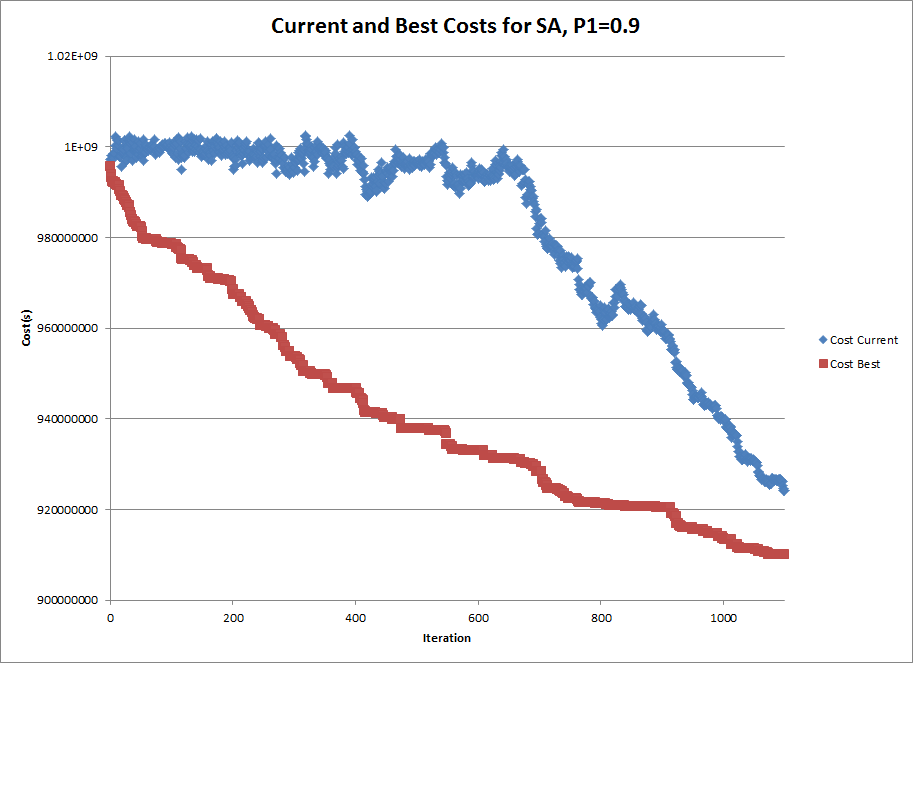
\includegraphics[width=\linewidth]{p1_09.png}
For these 30 trials, the average best cost after 1000 iterations was 913569927.986380, and the standard deviation among the trials was 23955996.148293. The average CPU time for the 30 trials was 0.009900 seconds.

\subsubsection{c}
When $P1 = 0.7$, $T_0 = -16113261.4/ln(0.7) = 45176320.0$, $\alpha = (-16113261.4/(45176320.0 * ln(0.05)))^{1/1000} = 0.997874$. Intuitively, $\alpha$ is greater because each temperature decrease step is less to move from probability 0.7 to 0.05 instead of 0.9 to 0.05.\\
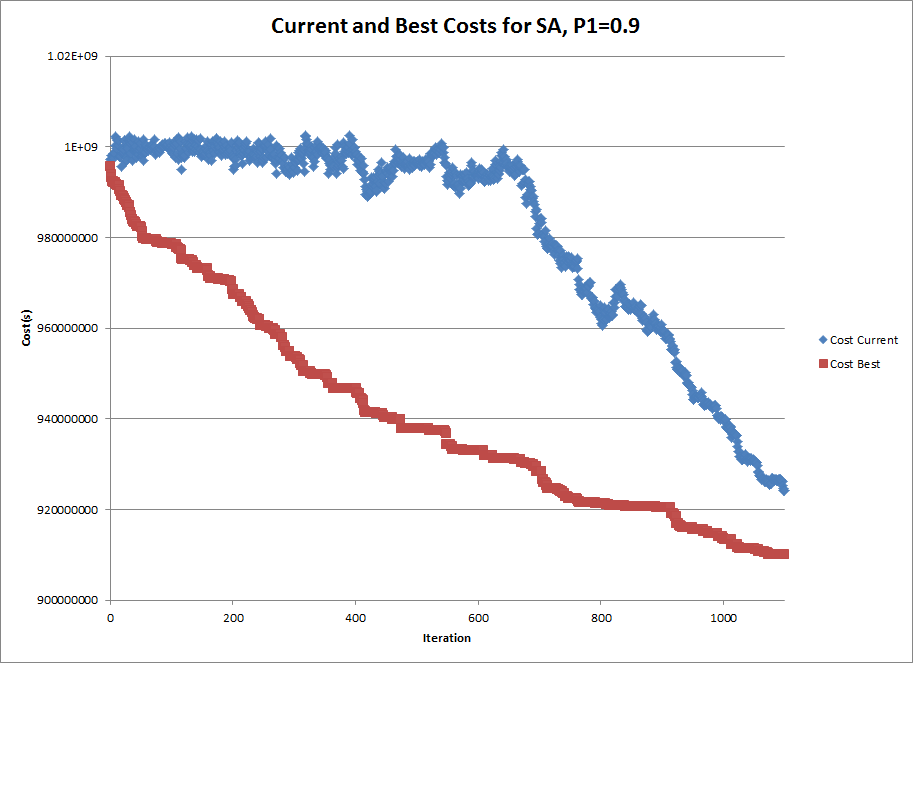
\includegraphics[width=\linewidth]{p1_09.png}
On these trials, the average best cost after 1000 iterations was 908484315.913066, the standard deviation was 22342227.133530, and the average CPU time was 0.008267 seconds.\\\\
Comparing after 1100 iterations, for $P1=0.9$, the average $BestCost=910015578.170673$, while for $P1=0.7$, the average $BestCost=907198602.927177$. In this set of 30 trials, $P1=0.7$ worked better than $P1=0.9$, as the best cost was lower.

\subsubsection{d}
On average, both sets of trials saw noticeable, although not large, improvements over the final 100 iterations. In the trial for P1=0.9, the average best cost decreased from 913569927.986380 to 910015578.170673, and in the trial for P1=0.7, the average best cost decreased from 908484315.913066 to 907198602.927177. Neither of these changes are dramatic on the scale of the cost, but they're enough to demonstrate a successful greedy finish to the simulated annealing algorithm.

\end{document}
